\section{Preliminaries}

%%%%%%%%%%%%%%%%%%%%%%%%%%%%%%%%%%%%%%%%%%%%%%%%%%%%%%%%%%%
\subsection{Questions we'd like to answer}

\bi

\i What distinguishes music from noise?

\i Why does a clarinet sound different from a flute?

%\i What is the harmonic series, and how is it related to
%  the analysis and synthesis of complex waves? 

\i Why do 10 violins sound only twice as loud as a single violin?

\i Why do you sound better when you sing in the shower?

\i Why do some notes harmonize while others clash?

\i What's equal temperament and why do we use it?

\i Others??

\ei

%%%%%%%%%%%%%%%%%%%%%%%%%%%%%%%%%%%%%%%%%%%%%%%%%%%%%%%%%
\subsection{Topics we will cover}

\bi

\i Preliminaries: basic math, physics, and music terminology

\i Physics of oscillations and waves

\i Production of sound (instruments, voice)

\i Perception of sound (hearing, loudness, pitch)

\i Room acoustics; reproduction and synthesis of 
sound

\i Musical scales and tuning systems

\ei
%%%%%%%%%%%%%%%%%%%%%%%%%%%%%%%%%%%%%%%%%%%%%%
\subsection{What is sound? What is music?}
\bi

\i Sound consists of pressure waves in air or 
in some other medium.
%(Can you produce a sound in the vacuum of space?)

\i Sounds are characterized by their loudness, 
duration, and pitch (if they have one).

\i Sounds can be measured and represented in
different ways:

(i) A {\em sound-level meter} measures the loudness or
intensity of a sound.

(ii) A {\em microphone attached to an oscilloscope} 
measures the pressure wave as
it changes in time (the waveform or shape of the wave).

(iii) A {\em spectrum analyzer} measures the different 
frequency components of the sound (high pitch, low pitch, 
or some combination).

(iv) A {\em spectrogram} shows how the frequency 
components of a sound change over time.

\i \demo 
Illustrate these different representations of sound using 
the Faber Electroacoustics Toolbox.

\i \demo
Illustrate the difference between a musical sound and
other sounds (e.g., noise) by looking at the various
representations of somebody speaking, singing, whistling;
play various instruments; have students applaud; crumple
a piece of paper, etc.

\i A musical note typically has a characteristic pitch
(fundamental frequency).
Hence, its associated pressure wave repeats over time.
Noise, on the other hand, doesn't have a characteristic pitch.

\i Not all sounds are within our range of hearing 
(the pitch might be too low or too high, or the 
sound might not be loud enough to hear).

\i \demo
Produce pure tones having different frequencies. 
Determine the range of frequencies that the class can
hear.
(The nominal range of human hearing is between 20~Hz and 
20,000~Hz.)

\i Ultrasound: sound waves whose frequencies lie {\em above}
the upper end of the audible range for humans.

\ex Dog whistle, echo-localization by bats,
non-ionizing medical imaging, sonograms ...

\i Infrasound: sound waves whose frequencies lie {\em below}
the lower end of the audible range for humans.

\ex Seismic waves, earthquakes, ...

\ei
%%%%%%%%%%%%%%%%%%%%%%%%%%%%%%%%%%%%%%%%%%%%%%
\subsection{Basic math review}

\bi

\i Basic operations:
Addition, subtraction, multiplication, division

\i Entering numbers on a calculator:
To evaluate $\frac{1}{2\pi}$, enter 
$1/(2\cdot \pi)$ and not $1/2\cdot \pi$.
The correct answer is 0.1592, not 1.5708.

\i Dividing fractions: 
Multiply by reciprocal---e.g.,
%
\be
\frac{2}{3/2}= 2\cdot \frac{2}{3} = \frac{4}{3}
\ee

\i Powers (exponential notation):

\be
2^4 = 2\cdot 2\cdot 2\cdot 2 = 16
\ee

\be
10^3 = 10\cdot 10\cdot 10 = 1000
\ee

\be
10^{-2} = \frac{1}{10^2} = .01
\ee

\i Prefixes:

\begin{center}
\begin{tabular}{|c|c|c|c|c|c|c|c|}
\hline
nano & micro & milli & centi & kilo & mega & giga & tera \\
\hline
$10^{-9}$ & $10^{-6}$ & $10^{-3}$ & $10^{-2}$ & $10^3$ & $10^6$ & $10^{9}$ & $10^{12}$ \\
\hline
\end{tabular}
\end{center}
%
For example, nanometer, centimeter, kilometer, millisecond, microsecond, etc.

\i Comparing two numbers: 
First need same units, then subtract, take ratio, or 
percent difference.

\i 
\ex I'm $5.5$~ft tall while Prof.~Borst is 72~in tall.

Convert units:
%
\be
5.5~{\rm ft}\cdot\frac{12\ {\rm in}}{1\ {\rm ft}} 
= 66~{\rm in}
\ee

Subtract: 
\be
72\ {\rm in}-66\ {\rm in}=6\ {\rm in}
\ee

Ratio: 
\be
\frac{72\ {\rm in}}{66\ {\rm in}}=1.09
\ee

Percent difference:
\be
\frac{72\ {\rm in}-66\ {\rm in}}
{66 {\rm in}} \cdot 100 
=9\%
\ee

Thus, one can say that Prof.~Borst is 6~inches taller 
than I am, 1.09 times taller than I am, or
9\% taller than I am.

\i 
In music, when comparing two numbers 
(e.g., frequencies or loudness levels),
using ratios is more convenient.

\ex We know that A$_2$ has a frequency
of 110~Hz (or 110~cycles/sec).
A$_3$ has a frequency of 220~Hz, 
which is twice that of A$_2$, or an octave higher.
A$_4$ has a frequency of 440~Hz, 
which is four times that of A$_2$, or two octaves higher.

\i Converting units:
multiply by the appropriate conversion factor written as
a fraction so that the unwanted units cancel out.
 
\i \exer How many centimeters are in a foot? 
(Use the conversion factor $1~{\rm in} = 2.54~{\rm cm}$.)

\ans
\be
1~{\rm ft} = 12~{\rm in}\cdot\frac{2.54~{\rm cm}}{1~{\rm in}} = 30.48~{\rm cm}
\ee

\i \exer Sound travels at $v_s=346~{\rm m/s}$ in dry air at a temperature
of $25~{}^\circ{\rm C}$.
Calculate the speed of sound in feet per second and miles per second.
(Use the conversion factors $1~{\rm m}=3.28~{\rm ft}$ and $1~{\rm mile} = 5280~{\rm ft}$.)

\ans
%
\be
v_s = 346~\frac{\rm m}{\rm s}\cdot \frac{3.28~{\rm ft}}{1~{\rm m}}
= 1135~\frac{\rm ft}{\rm s} 
\approx 1000~\frac{\rm ft}{\rm s}
\ee
%
\be
v_s = 1135~\frac{\rm ft}{\rm s}\cdot \frac{1~{\rm mile}}{5280~{\rm ft}}
= 0.21~\frac{\rm mi}{\rm s}
\approx \frac{1}{5}~\frac{\rm mile}{\rm s}
\ee
%

\i This last approximation allows us to estimate the distance 
to a thunderstorm if
we note the time between seeing a lightning strike and hearing the thunder.
(Light travels so fast ($3\times 10^8~{\rm m/s}$) 
that we see the lightning strike almost instantaneously.)
For example, if we hear thunder 5~seconds after we see a lightning strike, the
storm is approximately 1~mile away.

\ei
%%%%%%%%%%%%%%%%%%%%%%%%%%%%%%%%%%%%%%%%%%%%%%%%%%%
\subsection{Logarithms}
\bi

\i Since ratios of frequencies play such an important role 
in music, the mathematical concept of a logarithm is an
indispensible tool to have.

\i Logarithms:
%
\be
y = \log x 
\quad\Leftrightarrow\quad
x = 10^y
\ee

The above definition is for a base-10 logarithm,
$\log x = \log_{10}x$.

\i Since 
%
\be
10=10^1\,,\quad
100=10^2\,,\quad
1,000,000=10^6\,,\quad
1=10^0\,,\quad
0.001=10^{-3}
\ee
%
it follows that
%
\be
\log 10=1\,,\quad
\log 100=2\,,\quad
\log 1,000,000=6\,,\quad
\log 1=0\,,\quad
\log 0.001=-3
\ee
%
Thus,
%
\be
\log 10^n = n
\ee
%
which means that each multiplicative factor of 10 increase 
in $x$ corresponds to an additive increase of $y=\log x$ by 1. 
(See Figure~\ref{f:linear-log}.)
%
\begin{figure}[htbp]
\begin{center}
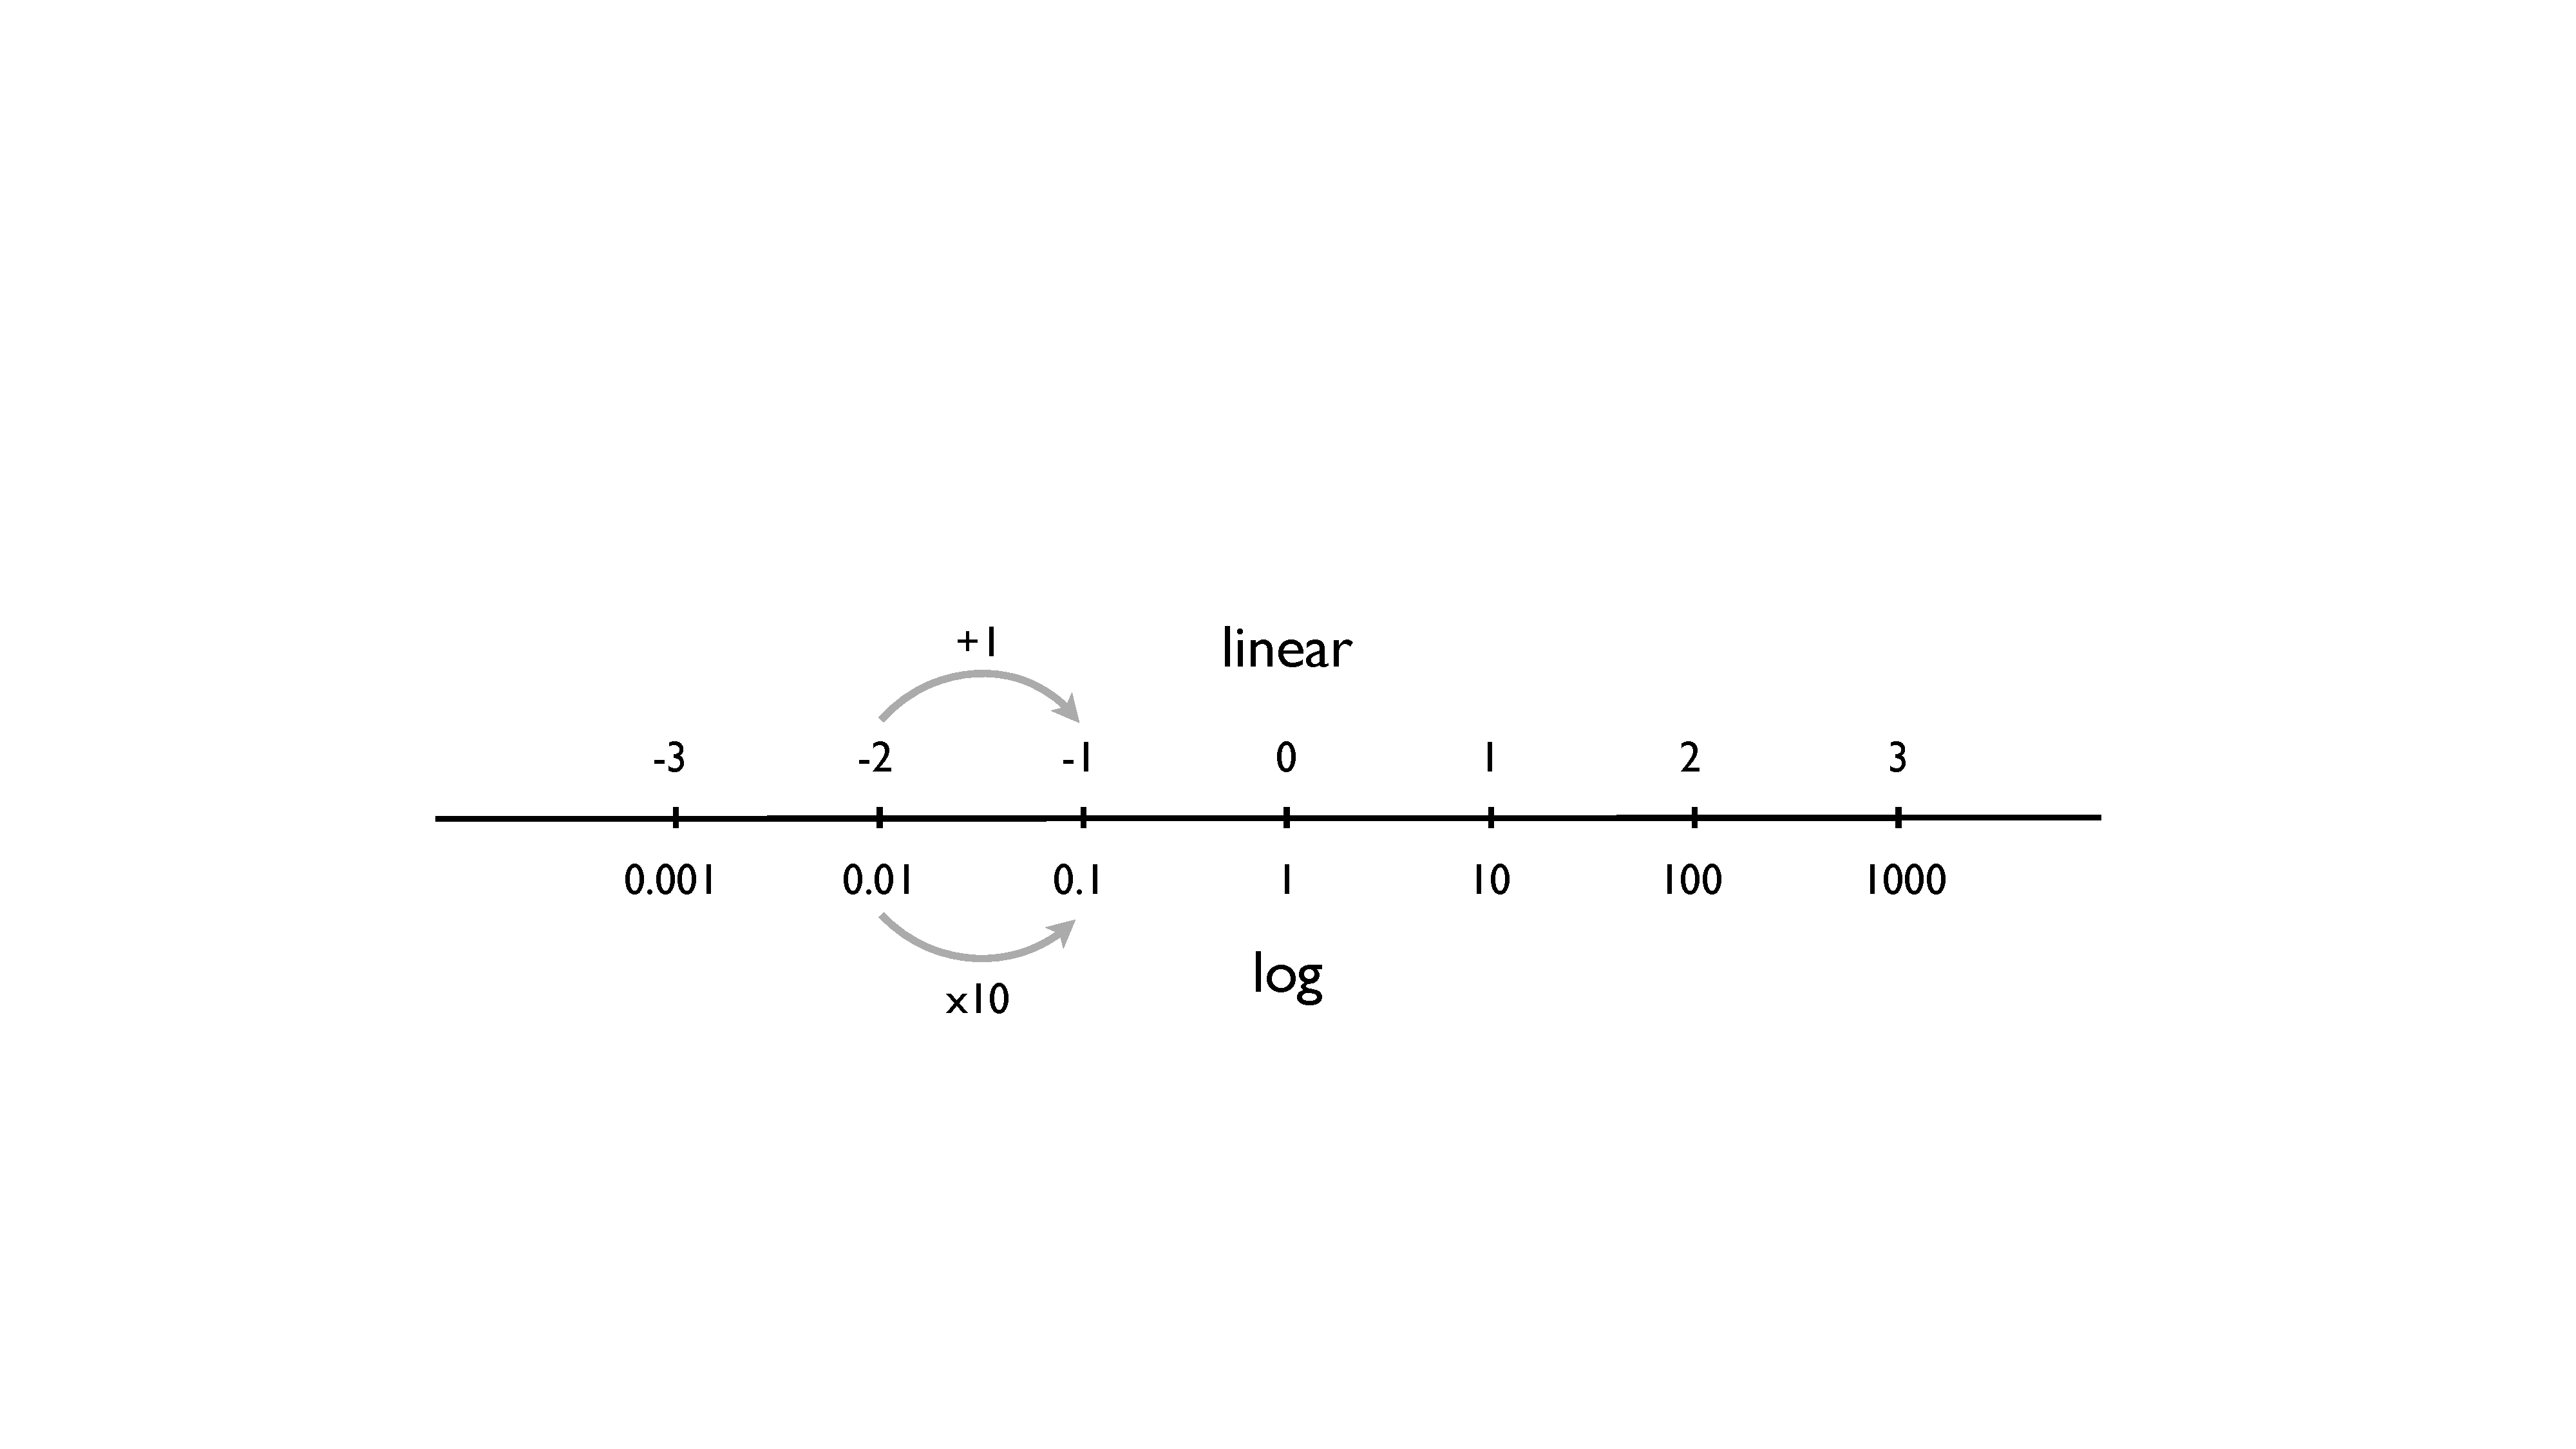
\includegraphics[width=.8\textwidth]{linear-log}
\caption{Difference between linear and logarithmic scales.
The tick marks on a linear scale are separated by a
constant additive term (here $+1$);
the tick marks on a logarithmic scale are separated by a
constant multiplicative factor (here $\times 10$).}
\label{f:linear-log}
\end{center}
\end{figure}
%

\i Key property of logarithms:
%
\be
\log(ab) = \log a + \log b\,,
\ee
%

\i Examples of logarithmic frequency scales:
Piano keyboard, musical staff, basilar membrane of the
human ear (which we shall describe later in the semester).

\i Equal divisions on the piano keyboard 
correspond to musical notes whose frequencies are related
by the same constant multiplicative factor---e.g., 
neighboring keys are 1 semitone apart, corresponding
to a frequency ratio of 
$2^{1/12}=1.05946$.
Thirteen keys on a piano keyboard are an octave apart, 
corresponding to a frequency ratio of 2.

\i Useful logarithms to remember:
%
\be
\log 2 \approx 0.3\,,\quad
\log 3 \approx 0.5\,,\quad
\log 4 \approx 0.6\,,\quad
\log 5 \approx 0.7\,,\quad
\log 10 = 1
\ee
%
Note that $\log 4 = \log(2\cdot 2) = 2\log 2$ and
$\log 5 = \log(10/2) = \log 10-\log 2$.

\ei

%%%%%%%%%%%%%%%%%%%%%%%%%%%%%%%%%%%%%%%%%%%%%%%%%%%%%%%%
\subsection{Music terminology}

\bi

\i Pitch: the fundamental frequency (i.e., the number 
of repetitions per second) of a musical note---e.g.,
concert A$_4$ has a fundamental frequency of 440~Hz.

\i Timbre: the distinctive quality or {\em color} of a
musical sound, which is due to the presence of overtones
or harmonics of the fundamental frequency.
(It's what distinguishes A$_4$ played on a piano and
A$_4$ played on a guitar.)

\i Interval: the separation or jump between two musical
notes, usually expressed as a ratio of the fundamental 
frequencies of the two notes.

\i Octave: a frequency interval corresponding to a factor 
of 2 difference in frequency.

\i Chromatic scale: a division of the octave into 12 
half-steps (or semitones).
Figure~\ref{f:chromatic-scale-keyboard} shows the
corresponding notes in a chromatic scale on 
a piano keyboard:
%
\be
{\rm C}-{\rm C}^\sharp-{\rm D}-{\rm E}^\flat-{\rm E}-%
{\rm F}-{\rm F}^\sharp-{\rm G}-{\rm A}^\flat-{\rm A}-%
{\rm B}^\flat-{\rm B}-{\rm C}'
\nonumber
\ee
%
\begin{figure}[htbp]
\begin{center}
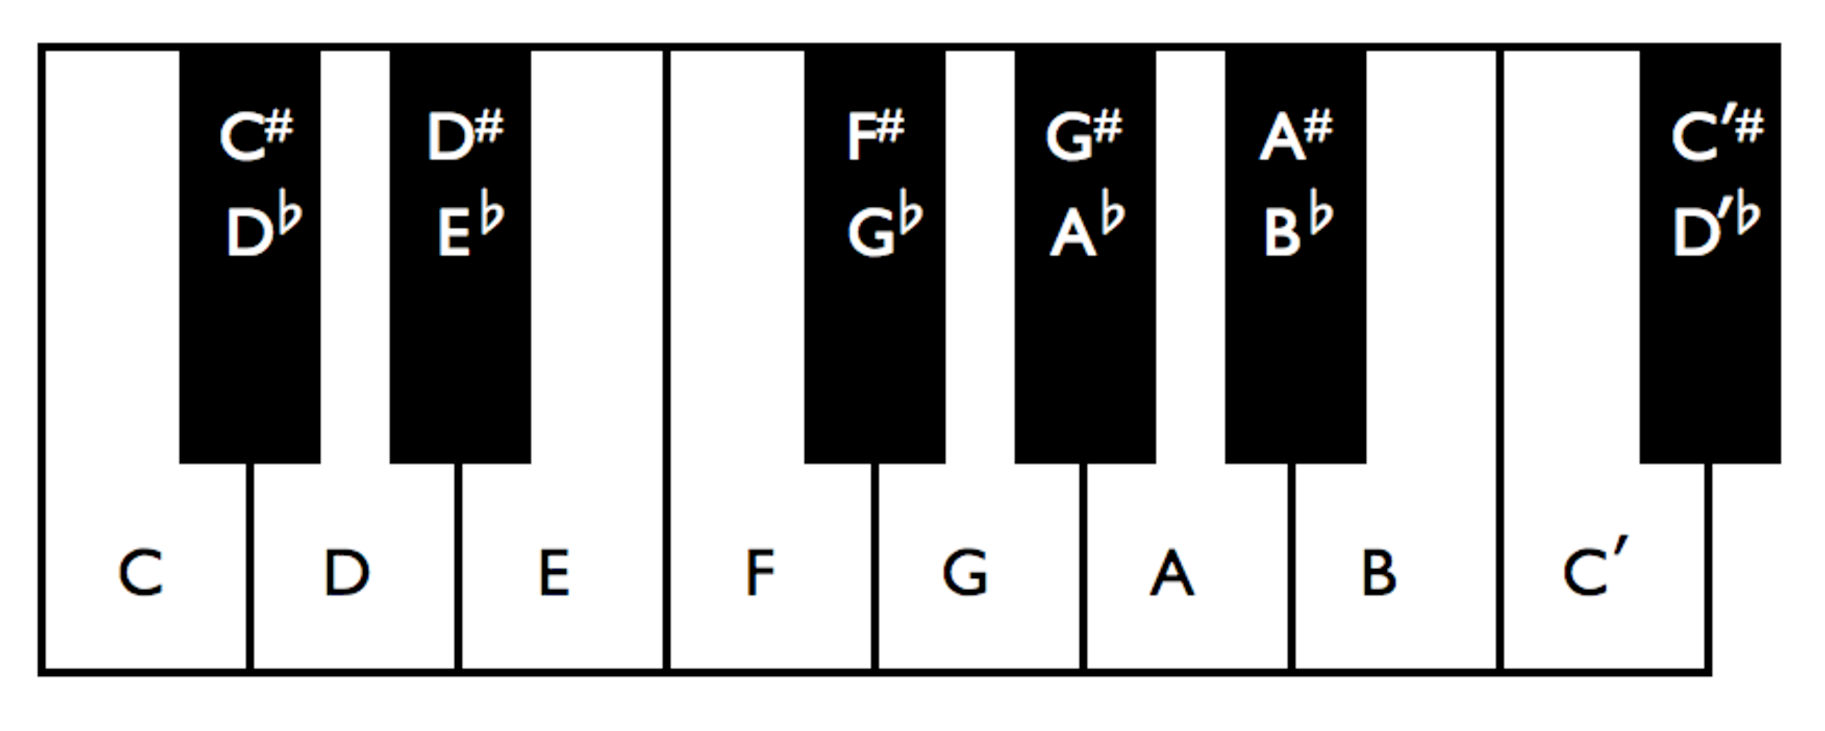
\includegraphics[width=.7\textwidth]{octave-keys}
\caption{Notes in a chromatic scale on a piano keyboard.}
\label{f:chromatic-scale-keyboard}
\end{center}
\end{figure}
%

\i Equal temperament: a tuning system for which all 
semitones in the octave have the same frequency ratio 
%
\be
2^{1/12}= 1.05946
\ee
In equal-temperament, the sharps and flats are equal
to one another---e.g., C${}^\sharp$ and D${}^\flat$
are tuned to the same frequency.
These are called {\em enharmonic} notes.

\i Diatonic scale: divides the octave into 
7 intervals consisting of both tones and semitones.
The order of tones and semitones 
defines the {\em major} and 
{\em minor} interval orders.

\i The diatonic major interval order is 
T-T-S-T-T-T-S (2-2-1-2-2-2-1).
This is the standard
%
\be
{\rm do-re-mi-fa-sol-la-ti-do}
\nonumber
\ee
%
interval order.

\i Fifth: a frequency interval corresponding to 
7 half-steps between two notes 
(e.g., C to G or A to E or B to F$^\sharp$).
The approximate frequency ratio of a fifth is $3/2=1.5$. 

\i Fourth: a frequency interval corresponding to
5 half-steps between two notes
(e.g., C to F or G to C).
The approximate frequency ratio of a fourth is $4/3=1.33$.

\i Major third: a frequency interval corresponding to 
4 half-steps between two notes 
(e.g., C to E or A to C$^\sharp$).
The approximate frequency ratio of a major third is $5/4=1.25$. 

\i Minor third: a frequency interval corresponding to 
3 half-steps (or semi-tones) between two notes 
(e.g., E to G or A to C).
The approximate frequency ratio of a minor third is $6/5=1.2$. 

\i Chord: three notes played simultaneously.
An example of a major chord is C-E-G (i.e., the tonic C
and the major third and fifth above C).
An example of a minor chord is C-E$^\flat$-G (i.e., the tonic C
and the minor third and fifth above C).

\ei

%%%%%%%%%%%%%%%%%%%%%%%%%%%%%%%%%%%%%%%%%%%%%%%%%%%%%%%%
\subsection{Physics terminology}

\bi

\i Position: 
the location of a point in space,
specified by the distance of that point away from a 
reference point, and a direction.
\\
Notation: $x$ or $y$
\\
Unit: meter, cm, inch, foot, ...

\i Displacement: 
the difference between two positions in space.
\\
Notation: $\Delta x$ or $\Delta y$ 
(which means {\em change} in $x$ or change in $y$)
\\
Unit: meter, cm, inch, foot, ...

\i Time: the reading on a clock.
\\
Notation: $t$
\\
Unit: second, minute, hour, ...

\i Duration (or time interval): 
the difference between two clock readings.
\\
Notation: $\Delta t$ (which means {\em change} in $t$).
\\
Unit: second, minute, hour, ...

\i Velocity: 
the rate of change of position with respect to 
time, which has both a magnitude and direction.
Notation:
%
\be
v= \frac{\Delta x}{\Delta t}
\ee
%
Unit: m/s, mile/hr (or mph), ...

In the absence of any outside influences, an object will either 
remain at rest or keep moving with the same velocity.

\i Speed: 
distance traveled per unit time. 
{\em Average} speed is the total distance traveled divided by
the total duration.
\\
Notation: $v$ 
\\
Unit: m/s, mile/hr (or mph), ...

\ex The speedometer needle in a car measures the instantaneous 
speed of the car.

\ex The speed of sound in dry air at a temperature of 
$25~{}^\circ{\rm C}$ is $v=346~{\rm m/s}$.

\i Acceleration: 
the rate of change of velocity with respect to 
time, which has both a magnitude and direction.
\\
Notation:
%
\be
a= \frac{\Delta v}{\Delta t}
\ee
%
Unit: ${\rm (m/s)/s} = {\rm m/s}^2$, mph/s, ...

\ex If my car accelerates from a stop sign at a 
constant rate of 10~mph/s, then after 6~seconds
I'll be traveling at 60~mph.

\ex A ball freely-falling toward the floor accelerates
at a constant rate of approximately $10~{\rm m/s}^2$.

\ex A weight attached to the end of a spring
oscillates vertically up and down with position, velocity,
and acceleration all changing with respect to time.
At the lowest and highest points, the velocity is zero,
while the acceleration has its maximum value (directed 
either upward or downward).
As the weight passes through the equilibrium position, 
the velocity has it maximum value (directed either upward
or downward), while the acceleration is zero.

\i Force: 
that which causes an object to accelerate.
A push or a pull. 
Gravity, electricity, and magnetism are examples of 
{\em non-contact} forces.
\\
Notation: $F$
\\
Unit: pound (lb), Newton (N)

\i Mass: 
the resistance that an object offers to changes in its state
of motion.
The larger the mass, the greater the force required to
get the same acceleration.
\\
Notation: $m$
\\
Unit: kilogram, gram, ...

\i Newton's 2nd law:
force, mass, and acceleration are related by the following formula:
%
\be
a = {F_{\rm net}}/{m} \quad
{\rm or,\ equivalently,}
\quad
F_{\rm net} = ma
\ee
%
where $F_{\rm net}$ is the {\em net} force (i.e., the sum of all forces) 
acting on the object.

\ex
The gravitational force exerted by the Earth on an object 
with mass $m$ is the object's weight and is given by 
%
\be
F_{\rm gravity}=mg
\ee
%
where $g=10~{\rm m/s}^2$ is the free-fall acceleration of
an object near the surface of the Earth.

\ex
The restoring force exerted by a spring stretched a distance
$x$ from its equilibrium position is given by {\em Hooke's law}:
%
\be
F_{\rm spring}=-kx
\ee
%
where $k$ is the spring constant, which tells how stiff the spring is.
The minus sign means that the force is directed back toward the 
equilibrium position.

\i Density:
the mass of an object divided by the volume occupied by the object.
\\
Notation: $\rho$
\\
Unit: ${\rm kg/m}^3$, ...

{\em Linear} mass density of a one-dimensional object like a guitar
string is given by the mass of the object divided by its length;
it has units of kg/m, ...

\ex The thicker guitar strings, which play the lower pitch (bass)
notes, have a larger linear mass density than the thinner strings.

\i Pressure:
force per unit area, where the force is perpendicular to the surface.
\\
Notation:
%
\be
P =\frac{F}{A}
\ee
%
where $A$ is the area over which the force is applied.

Unit: ${\rm N/m}^2= 1~{\rm Pa}$ (where Pa stands for Pascal) or
lb/in$^2$ (psi)

\ex Sound waves are pressure waves in air.

\ex On Earth, standard atmospheric pressure is approximately 
100~kPa, which is the same as $10^5~{\rm Pa}$.

\exer Calculate the pressure exerted by a 120~lb woman 
standing on the floor, 
wearing stilettos having an approximately circular 
heel with radius 0.25~in.
Compare that to the pressure exerted by a 
10,000~lb elephant,
whose feet are approximately circles with radius 10~in.

\ans

Woman:
%
\be
P = \frac{120\ {\rm lb}}{2 \cdot \pi \cdot (0.25~{\rm in})^2}
\approx 300~\frac{{\rm lb}}{{\rm in}^2}
\ee
%
%
Elephant:
%
\be
P = \frac{10000\ {\rm lb}}{4\cdot \pi \cdot (10~{\rm in})^2}
\approx 8~\frac{{\rm lb}}{{\rm in}^2}
\ee
%
So the pressure exerted by the woman's heels on the floor 
is almost 40 times greater than that exerted by the elephant!

\ei
